\documentclass{article}

\usepackage{fancyhdr} % Required for custom headers
\usepackage{lastpage} % Required to determine the last page for the footer
\usepackage{extramarks} % Required for headers and footers
\usepackage{graphicx} % Required to insert images
\usepackage[labelfont=bf, labelsep=space]{caption}
\usepackage{subcaption}
\usepackage{float}
\usepackage{lipsum} % Used for inserting dummy 'Lorem ipsum' text into the template
\usepackage{amsmath}
\usepackage{amssymb}
\usepackage{amsfonts}
\usepackage{hyperref}
\usepackage{titlesec}
\usepackage{listings}

% Margins
\topmargin=-0.45in
\evensidemargin=0in
\oddsidemargin=0in
\textwidth=6.5in
\textheight=9.0in
\headsep=0.25in 

\setcounter{secnumdepth}{4}

\titleformat{\paragraph}
{\normalfont\normalsize\bfseries}{\theparagraph}{1em}{}
\titlespacing*{\paragraph}
{0pt}{3.25ex plus 1ex minus .2ex}{1.5ex plus .2ex}

\linespread{1.1} % Line spacing

\DeclareMathOperator*{\argmax}{arg\,max}

\title{Unified variation discovery and genotyping from high throughput sequencing data: supplementary material}
\author{}
\date{}

\begin{document}

\maketitle

\tableofcontents

\section{Octopus}

\subsection{Overview}

Octopus is a general haplotype based method for calling variants in sequencing data samples generated from a range of biological sources and experimental designs. The core algorithm is the same regardless of the type of sample, but the various models and parameters of specific components are changed accordingly. Here we briefly go through the \emph{general} stages of the core variant calling algorithm. Each component will be explained in detail in the following sections.

The first step involved proposing \emph{task} (regions of the reference genome) to call. The reason for doing this rather than just calling the entire genome is to restrict memory consumption due to read buffering, and to facilitate multithreading. The basic steps are:

\begin{enumerate}
	\item Command line parameters are processed and checked. The calling model is deduced.
	\item Basic read statistics are calculated by taking random samples from across the input regions.
	\item A calling task is proposed by finding a subregion of the input regions that satisfies user given memory constraints. If multithreading is activated then a worker thread is spawned to do this task continually until the entire input region space is covered, tasks are added to a stack of tasks. Calling threads then take tasks from the stack and process them independently.
	\item For each task:
	\begin{enumerate}
		\item Fetch all reads for all samples from the input BAMs.
		\item Preprocess these reads \ref{read-preprocess}.
		\item Generate candidate \emph{alleles}. \ref{allele-generation}
		\item The algorithm then proposes an initial set of haplotypes \ref{haplotype-generation} using the candidate alleles, and proceeds to 'walk' across the task region sequentially until all candidate alleles are considered:
		\begin{enumerate}
			\item Calculate likelihoods for all haplotypes and all reads. \ref{haplotype-likelihood}
			\item Remove duplicate haplotypes \ref{haplotype-deduplication}
			\item Filter candidate haplotype with haplotype likelihoods. \ref{haplotype-likelihood-filtering}
			\item Evaluate all latent variables for the given calling model. \ref{calling-models}
			\item Filter candidate haplotype with inferred haplotype posteriors. \ref{haplotype-posterior-filtering}
			\item Propose the next set of candidate haplotypes. \ref{haplotype-generation}
			\item If there are any candidate alleles that were contained by the previous set of haplotypes but not the new set then these alleles are considered to have past and are elegible to be called. Candidate alleles are called by invoking the calling model with the latent variables previously inferred. \ref{calling-models}
			\item If any variants are called in the previous step then these are phased using the genotype posterior distribution inferred in the caller latent variables. \ref{phasing}
		\end{enumerate}
	\end{enumerate}
	\item Calls from each task are converted to VCF format, merged, and written.
	\item If variant filtering is requested then this is performed on the unfiltered VCF just written.
	\item If BAM realignments are requested then this is performed.
\end{enumerate}

\subsubsection{General notation and terminology}

Octopus distinguishes \emph{alleles} from \emph{haplotypes}. An allele is an atomic event; it is non-decomposable. Alleles are intended to represent single mutational events. On the other hand, haplotypes are simply non-overlapping sets of alleles.

We will usually denote a single haplotype with the letter $h$. Depending on the context, this could either mean the haplotypes sequence, or the set of alleles that define the haplotype.

\subsection{Read preprocessing}\label{read-preprocess}

Read preprocessing is intended to mitigate properties of reads that are not fully modelled and would therefore likely have detrimental consequences for calling accuracy and runtime. All of the preprocessing steps are optional.

\subsubsection{Read transformations}

Read transformations adjust the data contained in a read observation without removing the read. Most of the transformations recalibrate base qualities in certain ways. The current possible read transformations are:

\begin{center}
\begin{tabular}{ll}
Name & Description \\
\hline
Base quality cap & Caps the maximum base quality of all bases \\
Mask adapters & Sets base qualities of bases likely in adapter sequence to zero \\
Mask overlapping templates & Sets base qualities of bases overlapped by multiple templates from the same read segmenet to zero on all but one of the template \\
Mask low quality tails &  \\
Mask low quality soft clipped &  \\
\hline
\end{tabular}
\end{center}

\subsubsection{Read filtering}

Read filters remove reads that are likely problematic and cannot be transformed into something useful. Read filtering is applied \emph{after} read transformations. Reads are filtered if \emph{any} of the given filtering predicates fails. The current possible read filter predicates are:

\begin{center}
\begin{tabular}{ll}
Name & Description \\
\hline
Unmapped reads & Removes reads marked as unmapped \\
Min mapping quality & Removes reads with mapping quality less than a given threshold \\
Min good base quality fraction & Removes reads with a high fraction of low quality bases \\
QC fails & Removes reads marked as QC failed \\
Min read length & Removes short reads (e.g. due to hard clipping) \\
Max read length & Removes long reads \\
Marked duplicates & Removes reads marked as duplicates \\
Octopus duplicates & Removes reads identified as duplicates by Octopus \\
Secondary alignments & Removes reads marked as secondary alignments \\
Supplementary alignments & Removes reads marked as supplementary alignments \\
Adaptor contamination & Removes reads with likely adaptor contamination \\
\hline
\end{tabular}
\end{center}

\subsubsection{Read downsampling}

Read downsampling removes reads to satisfy user specified depth criteria. Sample read sets are downsampled independently. First, regions that have depth above a certain threshold are detected. Reads in these regions are then removed by iteratively sampling a read with weighting dependent on the remaining depth reduction criteria. Note that removing a read affects the depth at multiple positions (the original mapping and alignment are used). This process is run until no further positions have depth below the specified threshold.

\subsection{Candidate allele generation}\label{allele-generation}

Candidate allele generation is a crucial step for any variant caller as it sets an upper-bound on sensitivity. Ideally, the candidate generation stage should propose all true alleles whilst limiting the number of false alleles; too many false alleles is detrimental to runtime performance and can even have a negative impact on calling accuracy.

\subsubsection{Raw CIGAR scanner}

The raw CIGAR scanning allele generator is the simplest read-based generator. It uses the read mapping and alignment information present in the input BAM files and proposes candidates bases on mismatches present in these alignments. Alleles are only proposed if the observation of a particular satisfies some inclusion predicate, which primarily depends on the observation frequency; observed base qualities; and observation read strands. The inclusion predicate is fully parameterised so can be changed depending on the calling model (e.g. by lowering the observation frequency criteria for somatic calling).

\subsubsection{Repeat scanning}

The repeat scanner identifies common patterns of misalignments in microsatilities regions. In particular, it is common for reads fully or partially overlapping unique adjacent microsatilities to be aligned as a run of SNVs. However, our understanding of biology favours indels in these cases. By identifying run of SNVs the occur at regular intervals in microsatilities, this generator proposes indels which explain the observed read sequence. 

\subsubsection{Local re-assembly}

The local re-assembler generator is the most sophisticated allele generator. It completely discards read alignment information (but keeps mapping location) and builds an assembly (\emph{de Bruijn}) graph at regions considered likely to contain variation. Once the graph is constructed it is pruned to remove paths with low observation counts and cycles. Candidate alleles are extracted by enumerating the 'best' bubbles (divergent ref-non-reference paths).

\subsubsection{Input VCF}

This generator takes a set of user specified VCFs and extracts all alleles present in the region to be called. Filtering dependent on the QUAL of each site is optional.

\subsection{Haplotype generation}\label{haplotype-generation}

The \emph{haplotype generator} takes inputs reads and candidate alleles and generates sets of haplotypes. It is invoked multiple times, on each instance generating a new set of haplotypes. The subset of alleles that are included in the current set of haplotypes are considered \emph{active}. The input candidate alleles are gradually consumed until all have been active at least once. There are three important sub-components of the haplotype generator that dictate overall behaviour. 

\subsubsection{Dense region detector}

The dense region detector is used on construction to identify regions that would likely lead to serious runtime issues if fully processed. These are regions that have an extremely high candidate allele density and also abnormal coverage. They are almost certainly due to mapping errors. Depending on the level of confidence the a particular region is unsuitable for calling, the dense region detector recommends the region is either skipped entirely, or that haplotype lagging is disabled.

\subsubsection{Allele walker}

The allele walker takes the input reads, candidates, and the current set of active alleles, and proposes a new set of active alleles. Haplotypes are not considered. There are two important factors that influence how the next set of active alleles are proposed:

\begin{description}
	\item[Lagging] Determines how many of the current active alleles to include in the new set.
	\item[Extension] Determines how many new alleles to include.
\end{description}

Both factors influence how long haplotype can grow, and therefore determine the maximum achievable phase length. The lagging factor is especially crucial as this entirely determines whether or not alleles can be active more than once.

\subsubsection{Haplotype tree}

The haplotype tree is a data structure at the heart of Octopus. In this tree, nodes are candidate alleles and branches are haplotypes. Therefore, alleles along a branch are always ordered by genomic position and non-overlapping. The tree is unaware of the type of allele that is in the tree other than its genomic region footprint, therefore \emph{duplicate} haplotypes may be present in the tree; haplotypes that have identical sequence.

The haplotype tree supports three important operations that are the basis of Octopus' haplotype generation method:

\begin{description}
	\item[Extension] Extend all branches of the tree with new alleles.
	\item[Pruning] Remove certain branches while leaving others in place.
	\item[Rerooting] Change the root of the tree; removes nodes from near the trees root.
\end{description}

When Octopus filters haplotypes, it ultimately results in a request to prune certain branches of the current haplotype tree. By removing branches prior to extension, the growth rate of the tree can be controlled. Rerooting is required when alleles are passed over. For example, if the candidate allele set has alleles $\{A, B, C, D\}$ and the current tree has alleles $\{A, B, C\}$, the allele walker may propose the next set of alleles to be $\{B, C, D\}$. In this case the allele $A$ is no longer active so cannot appear in the next set of haplotypes, but $B$ and $C$ are still active, and may have had haplotypes containing them pruned from the tree. We want to maintain that information, which would be lost if we just reconstructed the complete tree for $\{B, C, D\}$. Rerooting shifts the root of the tree from being before $A$ to after $A$.

\subsection{Haplotype likelihood calculation}\label{haplotype-likelihood}

A haplotype likelihood is the probability that an observed read is generated from a sequencing machine assuming it originated from a known haplotype: $p(r | h, \mathcal{M}_{error})$. Read likelihoods in Octopus are computed with a paired hidden Markov Model (HMM).

\subsubsection{Kmer based re-mapping}\label{hmm:mapping}

The first step of the likelihood calculation is to remap the read $r$ to the given haplotype $h$. This is required because the HMM implementation which is responsable for calculating likelihoods has certain limitations that require the read be reasonably well placed before alignment, and the mapping position provided by the read mapper may not be accurate with respect to given haplotype. For example, if there are large indel alleles in the haplotype then this could shift the true mapping position.

We use a simple \emph{k-mer} based mapper to find putative mapping locations. Briefly, the k-mer ($k$ is hard coded) starting at each read and haplotype base are calculated. For each k-mer in the read we then see if that k-mer exists in the haplotype, and if it does, we calculate where in the haplotype the read should start assuming perfect alignment between the read and haplotype up until the k-mer (i.e. offset by the k-mer position in the read) and increment a 'hit' count at that position. After doing this for all k-mers in the read we look for positions in the haplotype that have high hit counts and emit these as putative mapping positions.

\subsubsection{Pair hidden Markov Model}

At the center of Octopus' haplotype likelihood calculate is a pair hidden Markov Model (pHMM). The pHMM likelihood method computes the approximate Viterbi probability of the read given the haplotype. We use the Viterbi probability rather than the forward probability since the Viterbi probability is considerably cheaper to compute in log space, and in practise the difference between the two calculations is small. The simplest pHMM implementation has positional gap open penalties which are a parameter to the model. There is a second version of the pHMM that also has so-called 'SNV' mismatch caps. This a vector of nucleotides and maximum base mismatch penalties, one for each position in the haplotype sequence, that limit the penalty of a mismatch aligned to that position where the mismatching read base is the nucleotide indicated in the provided vector. The intention of this is to model a common error mode in sequencing data in repetitive regions, especially homopolymers, where a single base on the edge of the repeat 'falls over' to the leading base of the repeat. We call these \emph{runthrough errors}. Runthrough errors are usually easily to detect with filtering as they are usually highly strand biased, but some level of modelling at the likelihood stage is an beneficial.

An important feature of our pHMM likelihood calculation is dubbed \emph{inactive flank score discounting}. To understand this calculation, it is important to remember that candidate haplotypes in Octopus are constructed from a set of candidate alleles (\ref{haplotype-generation}). However, it may be the cases that the true haplotype that a given read originates from is only partially formed in the set of candidate haplotypes. This can either be the case if the haplotype generator is yet to active an allele (i.e. the true allele is to the right of the current active set), or that the allele was deactivated and now lies to the left of the current active set. If this is the case, then the likelihood for a true haplotype could be lower than a false one just because the false one better support a true haplotype that has yet to be considered. This, in short, is the 'windowing' problem that all haplotype methods must address. Octopus' solution to the windowing problem is to only commit to calling candidate alleles once there is reasonable confidence that the reads supporting the alleles have had likelihoods evaluated on \emph{all} the true alleles they support. However, the problem still remains that we must evaluate the likelihood function with a haplotype that is correct in the active region, but false outside this region (sequences outside the active region are always padded with reference). To overcome this, we would like to 'discount' any reductions to the likelihood that arise from mismatches outside the active region. We do this by retracing the Viterbi path and subtract terms from the log likelihood that are due to mismatches outside the active region. In practice, we have found this approach is very effective. However, it is trivial to disable this feature.

The pHMM is a critical bottleneck in Octopus and is therefore uses a highly optimised banded SIMD implementation. By being banded, the likelihood calculation only explores a parts of the search space that imply an indel of more than the band size (currently 8). For short Illumina quality reads, this limitation is almost never an issue as indel \emph{errors} greater than this are extremely rare. For longer, noisier reads, the band size would need to be increased. Since the band size is just the width of the SIMD register used by the implementation (currently SSE2), to achieve a larger band size we would need to modify the code to use SIMD instructions that support larger register sizes (e.g. AVX2).

\subsubsection{Sequence error models}

Sequencing error models parameterise the likelihood HMM with indel gap open, gap extension, and optionally, SNV mismatch caps. The current implementation uses a constant gap extension penalty. The penalties are set according to local repeat context, up to some maximum repeat period (default 3 - trinucleotide repeats). There are currently two sequence error models: the default, which is intended for typical Illumina HiSeq quality data, and one intended for sequencing machines with higher error rates, such as the Illumina X Ten platform. We did not use any automated inference procedure to arrive at the parameters for these two models; we set them to reasonable values based on experience and observation.

\subsubsection{Considering mapping quality}

Mapping quality is an important mapping statistics that reflects the trustworthiness of a reads mapping location. Formally, it has been defined as the probability the read alignment is wrong. In Octopus, we are not so concerned with the \emph{alignment} of a read since all reads are realigned internally. However, if the read is incorrectly placed, to the degree that the remapping step (\ref{hmm:mapping}) cannot place the read correctly, then the read is not informative of the true haplotype and should not be used. 

\begin{align}
	p(r | h) &= p(r | h, \text{mapped})p(\text{mapped}) + p(r | h, \text{missmapped})p(\text{missmapped})\\
	         &= p(r | h, \text{mapped})q + p(r | h, \text{missmapped})(1 - q)
\end{align}

Where $q = 1 - 10^{\frac{-\text{MQ}(r)}{10}}$. $p(r | h, \text{mapped})$ is then simply the likelihood from the pHMM. $p(r | h, \text{missmapped})$ is a more interesting quantity. If the read is unmapped, then it originated from some other sequence not localised to the reference region used to construct the haplotype under consideration. There are three possibilities we must consider: i) The read originates from a region of the genome not included in the reference build. ii) The read originates from another genome (i.e. contamination). iii) The mapper made an error; the true mapping position in the reference build.

TODO

\subsection{Haplotype filtering}\label{haplotype-filtering}

A key operation in Octopus is removal of candidate haplotypes. Haplotype filtering can either come before genotype modelling or after. The latter is always preferable to the former.

\subsubsection{Deduplication}\label{haplotype-deduplication}

As described, the haplotype generator may propose haplotypes that have identical sequence but different allele compositions. These are called \emph{duplicates}. Duplicate haplotypes will have identical likelihoods, but may have different prior probabilities. This is because the alleles which make up the duplicates may have different probabilities under different models, but haplotype likelihoods are simply a function of the sequence.

Since duplicate haplotypes have the same likelihood, we can safety remove all but one duplicate with affecting the overall ranking of the other haplotypes under the genotype posterior distribution. In particular, if we move all but the duplicate with the highest prior probability under the same mutation model used by the callers genotype prior model, then we are guaranteed not to change the MAP genotype. We therefore remove duplicate haplotypes before genotype modelling, while keeping the one with the highest prior probability under the callers mutation model.

\subsubsection{Haplotype likelihood-based filtering}\label{haplotype-likelihood-filtering}

Haplotype likelihood filtering is required when the number of haplotypes is too large to be considered by the genotype model (as it would result in too many genotypes). To reduce the number of haplotypes, we calculate various likelihood based statistics designed to rank haplotypes by there chance of being true. It is important to recognise that this step has no information regarding the biological plausibility of certain configurations of haplotypes, or the frequency they may occur; it is entirely data driven. The statistics used are:

\begin{itemize}
	\item The maximum likelihood over all reads.
	\item The number of reads \emph{assigned} to each haplotype based on maximum likelihood.
	\item Number of likelihood zero reads; reads that have no recognisable sequencing errors.
\end{itemize}

In the first instance, we apply these filters with the condition that haplotypes are only filtered if there is a clear answer. In our experience, the first removes very few haplotypes but makes few errors. The second is the workhorse filter, and rarely removes a true haplotype. The last is error prone but is useful if the first two haven't removed the required number of haplotypes. If after apply all of these filters there are still haplotypes remaining then we rank haplotypes by the second statistic but force removal of some haplotypes that carry the same rank. Fortunately, in practise this is rarely required.

\subsubsection{Haplotype posterior-based filtering}\label{haplotype-posterior-filtering}

The posterior-based haplotype filter is the safest filter. It simply uses the haplotype posterior distribution inferred from the calling model to rank haplotypes. Haplotypes that have posterior probability below a certain threshold are filtered.

\subsection{Mutation models}

\subsubsection{Indel mutation model} \label{model:indel}

The indel mutation model assigns gap open and extension probabilities to a sequence at every position. It takes as input a basic rate parameter $r$, which is then scaled according to the local repeat composition of the sequence. For each position in a given haplotype $h$ we calculate the repeat period $period_i(h)$ and the numer of periods $len_i(h)$

The gap open probability for base $i$ is set according to the model described in Montgomery et al. The relative enrichment, which is scaled by the specified base rate is shown below for various period lengths.
 
\begin{figure*}[ht]
 \centering
 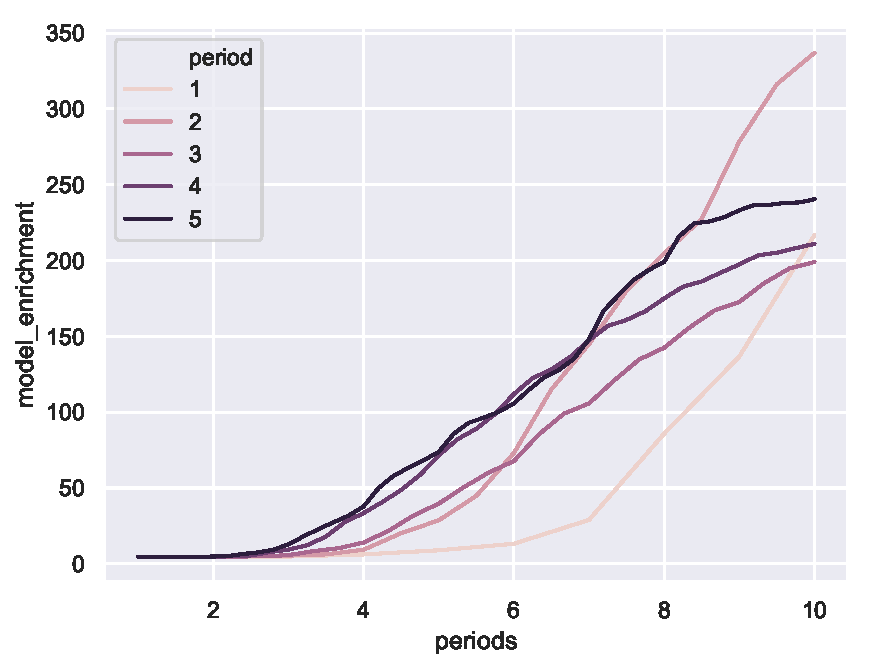
\includegraphics[width=0.9\textwidth]{figures/indel-open-model}
\end{figure*}

In addition to gap open probabilities, we also model gap extension penalties for each position along the sequence, dependent on the length of the current gap. The model is defined with the following Python code:

\begin{lstlisting}
	from math import exp, sqrt
	
	def sigmoid(x):
	    return 1 / (1 + exp(-x))
	
	def extension_model(period, periods, current_gap):
	    tract_length = period * periods
	    if periods > 1 and tract_length > 1:
	        if current_gap < tract_length:
	            if current_gap % period == 0:
	                return max(sigmoid(current_gap / period + min(sqrt(tract_length) - 3, 4)), extension_model(1, 1, current_gap))
	            else:
	                return 1.
	        else:
	            return extension_model(1, 1, current_gap - tract_length)
	    else:
	        return sigmoid(current_gap - 3)
\end{lstlisting}

A section of the model is shown in Figure \ref{indel-model:extension}. The most import aspect of the model is that the extension probability for repeat units is very high for between the unit length. This models the observation that indels in tandem repeats tend to occur in whole repeat units.

\begin{figure*}[ht]
	\label{indel-model:extension}
 \centering
 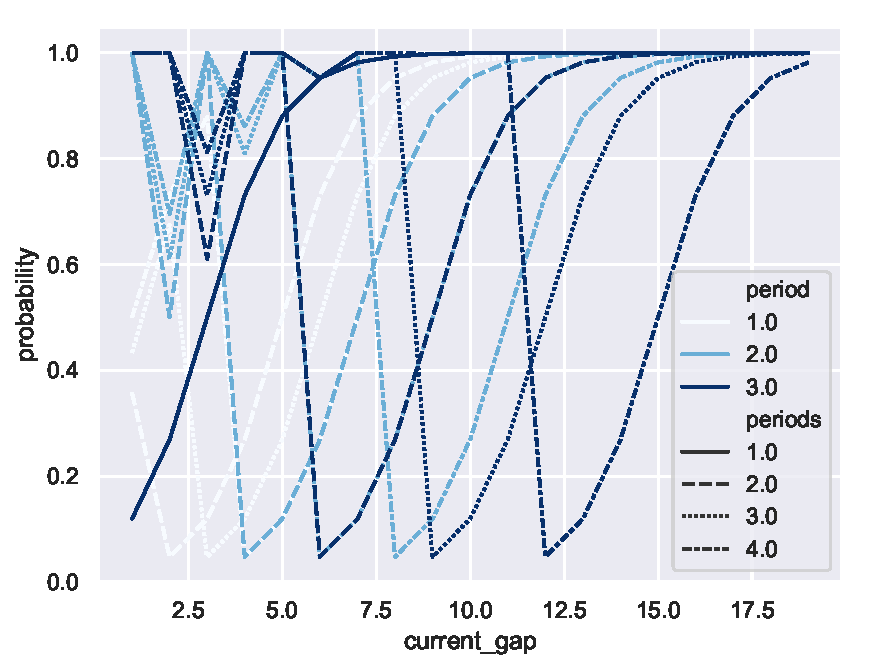
\includegraphics[width=0.9\textwidth]{figures/indel-extension-model}
\end{figure*}

\subsubsection{Coalescent mutation model}\label{model:coalescent}

The coalescent mutation model assigns probabilities to sets of haplotypes. The haplotypes are assumed to be sampled randomly from an idealised population.

There are two parameters to the model: $\theta_1$ is the SNV heterozygosity, $\theta_2$ is the indel heterozygosity. $\theta_1$ is set depending on user input. $\theta_2$ is set according the the indel mutation model \ref{model:indel} given the reference sequence and a user input indel heterozygosity value. The maximum indel gap open heterozygosity is used.

For a given set of haplotypes ${\boldsymbol{h} = \{h_1, \dots, h_m\}}$ we first calculate two quantities: $k_1$ is the number of unique segregating SNV sites observed in $\boldsymbol{h}$ and $k_2$ is the number of unique segregating indel sites observed in $\boldsymbol{h}$. Both values are calculated by comparing the alleles composing haplotypes to the reference haplotype. 

Probability is then assigned to $\boldsymbol{h}$ using the forumula:

\begin{equation}
    p(\boldsymbol{h} | \mathcal{M}_{coal}) = \binom{\theta_1}{\theta_1 + \theta_2}^{k_1} \binom{\theta_2}{\theta_1 + \theta_2}^{k_2} \binom{k_1 + k_2}{k_1} p_{\theta = \theta_1 + \theta_2} (k_1 + k_2)
\end{equation}

Where $p_\theta(S = k)\sum_{i=2}^n (-1)^i \binom{n - 1}{i - 1} \binom{i - 1}{\theta + i - 1} \binom{\theta}{\theta + i - 1}^k$. Which is an extension of formula $???$ found in John Wakeley's Coalescent theory.

We note a limitation of this model is that only a single indel heterozygosity value is used for all positions in the observed haplotypes. While this assumption is unrealistic, it turns out not to be particularly detrimental since the most important aspect of the model is to assign high likelihood to indels in repeat regions. The likelihood of proposing some other spurious indel in a region outside the repeat region is small given the haplotype lengths normally considered. We could look to address this issue in the future, particularly if the algorithm is updated to handle long-read data.

\subsubsection{De novo mutation model} \label{model:denovo-mutation}

The \textit{de novo} mutation model is intended assign probabilities to \textit{de novo} mutation occurring on a single haplotype during a single DNA replication. Formally, given an known haplotype $h_1$, the model assigns probabilities $p(h_2 | h_1)$ where $h_2$ is another haplotype (note that we can have $h_1$ = $h_2$). The model assigns probabilities according to the indel mutation model \ref{model:indel}, and a SNV mutation rate, that are parameters to the model.

\subsubsection{Somatic mutation model}\label{model:somatic-mutation}

The somatic mutation model assigns probabilities to somatic mutations occurring on a single haplotype over some time period. It is simply an instance of the \textit{de novo} mutation model \ref{model:denovo-mutation}.

\subsection{Genotype prior models}

Genotype prior models are used to assign prior probability to arrangements of genotypes. There are two types of genotype prior models: single and joint. Single genotype prior models assign probability to single genotypes, $p(g | \mathcal{M})$, joint genotype prior models assign probability to a \emph{combination} of genotypes, $p(\boldsymbol{g} | \mathcal{M})$. In some cases, such as the Coalescent genotype prior model, the former is simply a particular instance of the first, although it may have a separate implementation for efficiency. We report the unnormalised versions of each genotype prior model since normalisation is trivial, and is always performed as part of the genotype posterior model in any case (there is no need to report normalised genotype priors).

\subsubsection{Uniform genotype prior model}\label{model:uniform}

The uniform genotype prior model, $\mathcal{M}_{uni}$, is the simplest genotype prior model. We have:

\begin{equation}
    p(g | \mathcal{M}_{uni}) = 1
\end{equation}

for the single case, and:

\begin{equation}
    p(\boldsymbol{g} | \mathcal{M}_{uni}) = 1
\end{equation}

for the joint case.

\subsubsection{HWE genotype prior model}\label{model:hwe}

The Hardy-Weinberg Equilibrium (HWE) genotype prior model, $\mathcal{M}_{hwe}$, assigns probability to genotypes assuming HWE. The model is paramertised by a set of known haplotypes $\boldsymbol{h} = \{h_1, \dots, h_m\}$, and their frequencies, $f_i$ (for $i = 1 to m$). The haplotype frequencies may be set explicitly, or calculated with empirical Bayes. We recall the the HWE is simply a multinomial distribution:

\begin{equation}
    p(g | \mathcal{M}_{hwe}) = \binom{|g|}{o_1(g), \dots, o_m(g)} \prod_{i=1}^m f_i^{o_i(g)}
\end{equation}

where $o_i(g)$ is the number of times haplotype $i$ occurs in genotype $g$.

\subsubsection{Coalescent-HWE genotype prior model}\label{model:coalescent-hwe}

The coalescent-HWE genotype prior model, $\mathcal{M}_{coal-hwe}$, is suitable for modelling germline genotypes; it is the default germline prior model for all calling models. There are two components to this model: a \emph{segregation} model, that assigns probability to the pattern of observed alleles in the genotype(s); and a \emph{frequency} model that assigns probability to the frequency each haplotype is observed. In particular, the segregation model is just the coalescent mutation model (\ref{model:coalescent}) and the frequency model is a Hardy-Weinberg model (\ref{model:hwe}) parameterised with empirical Bayes. We then have:

\begin{equation}
    p(\boldsymbol{g} | \mathcal{M}_{coal-hwe}) = p(\boldsymbol{g} | \mathcal{M}_{coal}) p(\boldsymbol{g} | \mathcal{M}_{hwe})
\end{equation}

for the joint case. The individual case can be optimised to

\begin{equation}
    p(g | \mathcal{M}_{coal-hwe}) = p(g | \mathcal{M}_{coal})
\end{equation}

when $|g| \le 2$ (i.e. the sample is haploid or diploid) since $p(g | \mathcal{M}_{hwe})$ is then constant.

\subsubsection{Trio genotype prior model}\label{model:trio-prior}

The trio genotype prior model, $\mathcal{M}_{trio}$, assigns probabilities to triplets of genotypes that originate from parent-offspring trios. This model encapsulates two elements of uncertainty: inheritance patterns and parental haplotype modification due \textit{de novo} mutations. The model uses Coalescent-HWE genotype prior model (\ref{model:coalescent-hwe}) or uniform prior model (\ref{model:uniform}) to assign probability to parental genotypes and the \emph{de novo} mutation model (\ref{model:denovo-mutation}) to model modifications to parental haplotypes. Let $g_m$, $g_p$, $g_o$ be the maternal, paternal, and offspring genotypes, respectively. This model then calculates $p(g_m, g_p, g_o | \mathcal{M}_{trio})$.

\begin{equation}
    p(g_o, g_m, g_p | \mathcal{M}_{trio} = (\mathcal{M}_{germline}, \mathcal{M}_{denovo})) = p(g_m, g_p | \mathcal{M}_{germline}) p(g_o | g_m, g_p, \mathcal{M}_{denovo})
\end{equation}

The form of the latter term $p(g_o | g_m, g_p, \mathcal{M}_{denovo})$ is dependent on meiosis and fertilisation in the species under consideration. We only consider the mammalian case here.

Writing $\mathcal{M}_{d} \equiv \mathcal{M}_{denovo}$ for brevity. In the autosomal (i.e. all diploid) case, we have

\begin{align}
    p(g_o | g_m, g_p, \mathcal{M}_{d}) &= \frac{1}{2} p(g_{o0} | g_m, \mathcal{M}_{d})p(g_{o1} | g_p, \mathcal{M}_{d}) \\ &+ \frac{1}{2} p(g_{o1} | g_m, \mathcal{M}_{d}) p(g_{o0} |g_p, \mathcal{M}_{d})
\end{align}

reflecting the uncertainty in parental origin of the offspring haplotypes, and where

\begin{equation}
p(g_{oi} |g_s, \mathcal{M}_{d}) = \frac{1}{2} p(g_{oi} | g_{s0}, \mathcal{M}_{d}) + \frac{1}{2} p(g_{oi} | g_{s1}, \mathcal{M}_{d})
\end{equation}

models uncertainty in which parental haplotype is inherited. $p(g_{oi} | g_{sj}, \mathcal{M}_{d})$ is the probability the haplotype $g_{oi}$ is inherited by the child given that the haplotype $g_{sj}$ is the one provided by the parent $s$ for fertilisation; it models \textit{de novo} mutations.

For the female offspring X chromosome case we have the same form for $p(g_o | g_m, g_p, \mathcal{M}_{d})$ as the autosomal case, but

\begin{equation}
p(g_{oi} | g_p, \mathcal{M}_{d}) = p(g_{oi} | g_{s0}, \mathcal{M}_{d})
\end{equation}

For the male offspring X chromosome case we have

\begin{equation}
 p(g_o | g_m, g_p, \mathcal{M}_{d}) = p(g_{o0} | g_m, \mathcal{M}_{d})
\end{equation}

Finally, in the male offspring Y chromosome case we simply have

\begin{equation}
 p(g_o | g_m, g_p, \mathcal{M}_{d}) = p(g_{o0} | g_{p0}, \mathcal{M}_{d})
\end{equation}

\subsubsection{Cancer genotype prior model}\label{model:cancer-prior}

The cancer genotype prior model, $\mathcal{M}_{cancer}$, is used to assign probability to \emph{cancer genotypes}. A cancer genotype is a pair of regular genotypes, $g_{cancer} = (g_{germline}, g_{somatic})$, where $g_{germline}$ is the germline and $g_{somatic}$ is acquired somatically. The model must explain both the germline and the somatic genotypes. Note that no assumptions of either germline or somatic genotype ploidy are made.

The model $\mathcal{M}_{cancer}$ is can be seen as the composition of two independent models: a germline prior model, $\mathcal{M}_{germline}$ (e.g. the coalescent-HWE model (\ref{model:coalescent-hwe})); and a \emph{conditional somatic model}, $\mathcal{M}_{somatic}$. We can then write

\begin{equation}
 p(g_{cancer} | \mathcal{M}_{cancer} = (\mathcal{M}_{germline}, \mathcal{M}_{somatic})) = p(g_{germline} | \mathcal{M}_{germline}) p(g_{somatic} | g_{germline}, \mathcal{M}_{somatic})
\end{equation}

The second term $p(g_{somatic} | g_{germline}, \mathcal{M}_{somatic})$ is of most interest, as it models the \emph{pattern} of somatic haplotypes. In the simplest case when $|g_{somatic}| = 1$ (i.e. there is a single somatic haplotype) then we just have

\begin{equation}
	\label{eq:single-somatic}
	p(g_{somatic} | g_{germline}, \mathcal{M}_{somatic}) = \frac{1}{|g_{germline}|} \sum_{i = 1}^{|g_{germline}|} p(g_{somatic,0} | g_{germline, i}, \mathcal{M}_{somatic})
\end{equation}

where $p(g_{somatic,0} | g_{germline, i}, \mathcal{M}_{somatic})$ is just the probability of observing the somatic haplotype given the germline haplotype $g_{germline, i}$ suffers some mutational event (which in theory could lead to the same sequence); it is just the somatic mutation model (\ref{model:somatic-mutation}).

What is more interesting is when $|g_{somatic}| > 1$ (i.e. there are more than one somatic haplotypes). In principle, we must consider that any of the somatic haplotypes could have originated from either the germline \emph{or any other somatic haplotype}. That is, this probability should consider possible tumour phylogenies. Unfortunately, we have not implemented such a model in Octopus; instead we just assume independence between somatic haplotypes:

\begin{equation}
p(g_{somatic} | g_{germline}, \mathcal{M}_{somatic}) = \prod_{j = 1}^{|g_{somatic}|} p(g_{somatic,j} | g_{germline}, \mathcal{M}_{somatic})
\end{equation}

where $p(g_{somatic,j} | g_{germline}, \mathcal{M}_{somatic})$ is calculated as in (\ref{eq:single-somatic}).

\subsection{Genotype posterior models}\label{model:genotype-posterior}

non-referencehough each genotype model is in a sense independent, they do share common attributes which we define here for brevity.

\begin{center}
\begin{tabular}{ll}
Constants & Description \\
\hline
$P_s$ & The ploidy of organism $s$\\
$h$ & A haplotype \\
$\mathbb{M_{e}}$ & The sequencing error model \\
\hline
\end{tabular}
\end{center}

\begin{center}
\begin{tabular}{ll}
Observed variables & Description \\
\hline
$r$ & A sequencing read \\
\hline
\end{tabular}
\end{center}

Then the conditional probability of a read given a haplotype is:

\begin{equation}
\label{eq:read_prob}
    p(r | h, \mathbb{M_{e}})
\end{equation}

Which has already been described. For brevity, we will from here on omit the $\mathbb{M_{e}}$ term and just write $p(r | h)$.

\subsubsection{Individual}\label{genotype-model:individual}

This model is designed to model reads coming from a single individual with a known fixed ploidy. It is the simplest genotype model that Octopus offers, and is also the fastest to compute. It is used by multiple Octopus variant callers.

\begin{figure*}[ht]
    \centering
    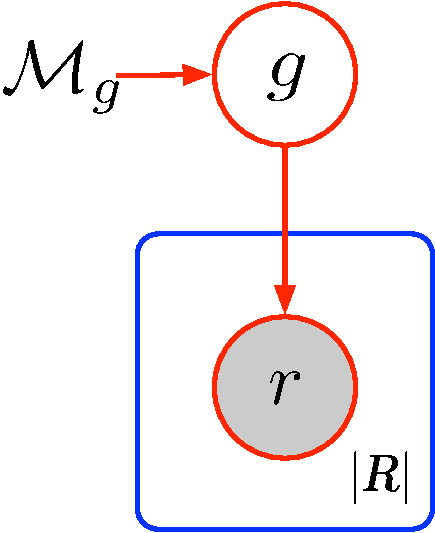
\includegraphics[width=0.3\textwidth]{figures/individual_model}
\end{figure*}

\paragraph{Definitions}

\begin{center}
\begin{tabular}{ll}
Constants & Description \\
\hline
$P$ & The individuals ploidy \\
$G$ & The number of genotypes \\
$\boldsymbol{\phi}$ & Vector of $G$ probabilities \\
$h_{ij}$ & The $j^{th}$ haplotype of the $i^{th}$ genotype \\
$\mathcal{R}$ & The set of sequencing reads for the individual \\
$N$ & $\mathcal{R}$ \\
\hline
\end{tabular}
\end{center}

Note that $h_{ij}$ is technically a deterministic surjective function $h_{ij} = f(\boldsymbol{g}, i, j)$ which maps genotypes to haplotypes, but for brevity we just write $h_{ij}$.

\begin{center}
\begin{tabular}{ll}
Observed variables & Description \\
\hline
$\mathcal{R}$ & The set of sequencing reads for the individual \\
$N$ & $\mathcal{R}$ \\
\hline
\end{tabular}
\end{center}

\begin{center}
\begin{tabular}{ll}
Latent variables & Description \\
\hline
$\boldsymbol{g}$ & Binary (1-of-$G$) \\
\hline
\end{tabular}
\end{center}

\paragraph{Prior distributions}

There is just one prior in this model, the genotype prior:

\begin{equation}
    p(\boldsymbol{g} | \boldsymbol{\phi}) = \prod_{i = 1}^G \phi_i^{g_i}
\end{equation}

Where the $\phi_i^{g_i}$ is set according to some genotype prior model (e.g. the coalescent genotype prior model).

\paragraph{Marginal distributions}

The marginal distribution for $\boldsymbol{g}$ is categorical:

\begin{equation}
\label{eq:ind_g_marginal}
    p(\boldsymbol{g} | \boldsymbol{\phi}) = \prod_{i = 1}^G \phi_i^{g_i}
\end{equation}

The marginal distribution for a single read $r$ is a mixture distribution, which follows from the assumption that the haplotypes that make up a known ploidy genotype are exchangeable, and thus we must assign them equal probabilities of being sequenced:

\begin{equation}
\label{eq:ind_read_marginal}
 p(r | g_i = 1) = \frac{1}{P} \sum^P_{k = 1} p(r | h_{ik})
\end{equation}

which can also be written as:

\begin{equation}
\label{eq:ind_read_marginal2}
 p(r | \boldsymbol{g}) = \prod_{i = 1}^G \frac{1}{P} \sum^P_{k = 1} p(r | h_{ik})^{g_i}
\end{equation}

\paragraph{Joint distribution}

\begin{equation}
\label{eq:ind_jp}
 p(\mathcal{R}, \boldsymbol{g}) = \prod_{i = 1}^G \phi_i^{g_i} \prod^N_{n = 1} \frac{1}{P} \sum^P_{k = 1} p(r_n | h_{ik})^{g_i}
\end{equation}

\paragraph{Posterior distribution}

\begin{equation}
\label{eq:ind_post}
 p(\boldsymbol{g} | \mathcal{R}) = \frac{\prod_{i = 1}^G \phi_i \prod^N_{n = 1} \frac{1}{P} \sum^P_{k = 1} p(r_n | h_{ik})^{g_i}}{\sum_{\boldsymbol{g}'}\prod_{i = 1}^G \phi_i \prod^N_{n = 1} \frac{1}{P} \sum^P_{k = 1} p(r_n | h_{ik})^{g_i}}
\end{equation}

We can factor out the constant $P$ term, and write more compactly as:

\begin{equation}
\label{eq:ind_post2}
 p(g_i = 1 | \mathcal{R}) = \frac{\phi_i \prod^N_{n = 1} \sum^P_{k = 1} p(r_n | h_{ik})}{\sum_{j = 1}^G \phi_j \prod^N_{n = 1} \sum^P_{k = 1} p(r_n | h_{jk})}
\end{equation}

\paragraph{Evidence}

The evidence for the model is simply the denominator of (\ref{eq:ind_post}):

\begin{equation}
\label{eq:ind_ev}
 p(\mathcal{R}) = \sum_{i = 1}^G \phi_i \prod^N_{n = 1} \frac{1}{P} \sum^P_{k = 1} p(r_n | h_{ik})
\end{equation}

\subsubsection{Population}

\begin{figure*}[ht!]
    \centering
    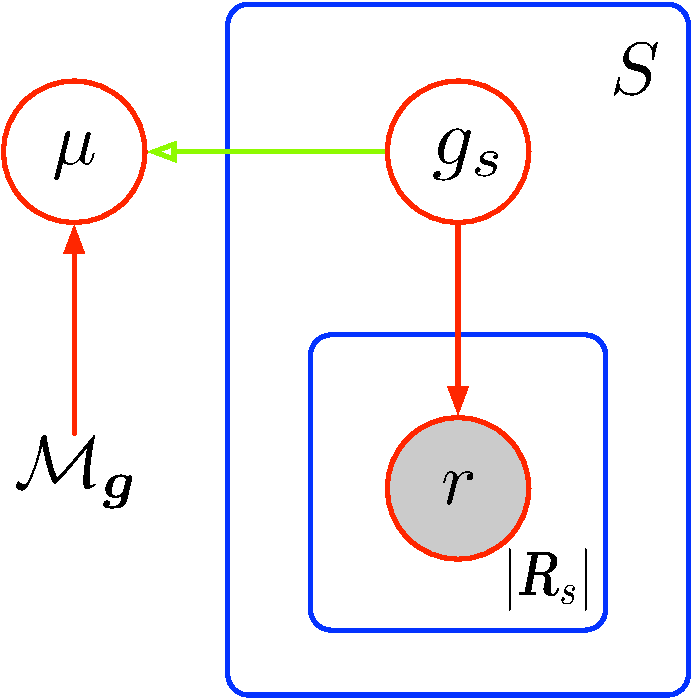
\includegraphics[width=0.3\textwidth]{figures/population_model}
\end{figure*}

\paragraph{Definitions}

\paragraph{Prior distributions}

\paragraph{Marginal distributions}

\paragraph{Joint distribution}

\paragraph{Posterior distribution}

\paragraph{Evidence}

\subsubsection{Trio}\label{model:trio}

\begin{figure*}[ht]
    \centering
    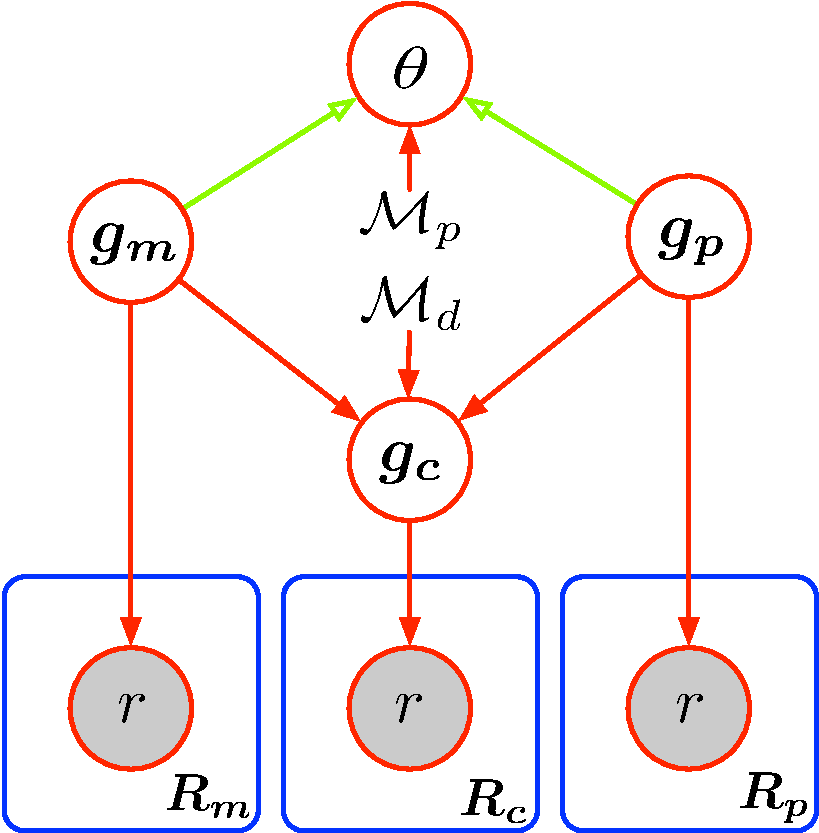
\includegraphics[width=0.3\textwidth]{figures/trio_model}
\end{figure*}

\paragraph{Definitions}

\begin{center}
\begin{tabular}{ll}
Constants & Description \\
\hline
$P_s$ & The ploidy for individual $s$ \\
$G_s$ & The number of genotypes for individual $s$ \\
$\boldsymbol{\phi}$ & 3D tensor ($G_m,G_p,G_o$) of genotype probabilities for the trio \\
$h_{sij}$ & The $j^{th}$ haplotype of the $i^{th}$ genotype for sample $s$ \\
\hline
\end{tabular}
\end{center}

\begin{center}
\begin{tabular}{ll}
Observed variables & Description \\
\hline
$\boldsymbol{\mathcal{R}}$ & The set of sequencing reads for the trio \\
$\mathcal{R}_s$ & The set of sequencing reads for sample s \\
\hline
\end{tabular}
\end{center}

\begin{center}
\begin{tabular}{ll}
Latent variables & Description \\
\hline
$\boldsymbol{g}_m$ & Binary (1-of-$G_m$) \\
$\boldsymbol{g}_p$ & Binary (1-of-$G_p$) \\
$\boldsymbol{g}_o$ & Binary (1-of-$G_o$) \\
$\boldsymbol{g}$ & $(\boldsymbol{g}_m, \boldsymbol{g}_p, \boldsymbol{g}_o)$ \\
\hline
\end{tabular}
\end{center}

\paragraph{Prior distributions}

\begin{equation}
    p(\boldsymbol{g} | \boldsymbol{\phi}) = \prod_{i = 1}^{G_m}\prod_{j = 1}^{G_p}\prod_{k = 1}^{G_o} \phi_{ijk}^{g_{mi} g_{pj} g_{ok}}
\end{equation}

\paragraph{Marginal distributions}

\begin{equation}
 p(\boldsymbol{g} | \boldsymbol{\phi}) = \prod_{i = 1}^{G_m}\prod_{j = 1}^{G_p}\prod_{k = 1}^{G_o} \phi_{ijk}^{g_{mi} g_{pj} g_{ok}}
\end{equation}

\begin{equation}
 p(r | g_{si} = 1) = \frac{1}{P_s} \sum^{P_s}_{k = 1} p(r_s | h_{sik})
\end{equation}

\paragraph{Joint distribution}

\begin{equation}
 p(\mathcal{R}, \boldsymbol{g}) = \prod_{i = 1}^{G_m}\prod_{j = 1}^{G_p}\prod_{k = 1}^{G_o} \phi_{ijk}^{g_{mi} g_{pj} g_{ok}} \prod_{s \in \{m, p, o \}} \prod^{N_s}_{n = 1} \frac{1}{P_s} \sum^{P_s}_{l = 1} p(r_s | h_{sil})^{g_{mi} g_{pj} g_{ok}}
\end{equation}

\paragraph{Posterior distribution}

\begin{equation}
 p(\boldsymbol{g} | \mathcal{R}) = \frac{\prod_{i = 1}^{G_m}\prod_{j = 1}^{G_p}\prod_{k = 1}^{G_o} \phi_{ijk}^{g_{mi} g_{pj} g_{ok}} \prod_{s \in \{m, p, o \}} \prod^{N_s}_{n = 1} \frac{1}{P_s} \sum^{P_s}_{k = 1} p(r_s | h_{sik})^{g_{mi} g_{pj} g_{ok}}}{\sum_{\boldsymbol{g}_m} \sum_{\boldsymbol{g}_p} \sum_{\boldsymbol{g}_o} \prod_{i = 1}^{G_m}\prod_{j = 1}^{G_p}\prod_{k = 1}^{G_o} \phi_{ijk}^{g_{mi} g_{pj} g_{ok}} \prod_{s \in \{m, p, o \}} \prod^{N_s}_{n = 1} \frac{1}{P_s} \sum^{P_s}_{l = 1} p(r | h_{sil})^{g_{mi} g_{pj} g_{ok}}}
\end{equation}

Which we can write more compactly as

\begin{equation}
 p(g_{mi} = 1, g_{pj} = 1, g_{ok} = 1 | \mathcal{R}) = \frac{\phi_{ijk}  \prod_{s \in \{m, p, o \}} \prod^{N_s}_{n = 1} \sum^{P_s}_{k = 1} p(r_{sn} | h_{ik})}{\sum_{i' = 1}^{G_m} \sum_{k' = 1}^{G_p} \sum_{k' = 1}^{G_o} \phi_{i'j'k'} \prod_{s \in \{m, p, o \}} \prod^{N_s}_{n = 1} \sum^{P_s}_{l = 1} p(r_{sn} | h_{il})}
\end{equation}

\paragraph{Evidence}

\begin{equation}
 p(\mathcal{R}) = \sum_{i' = 1}^{G_m} \sum_{k' = 1}^{G_p} \sum_{k' = 1}^{G_o} \phi_{i'j'k'} \prod_{s \in \{m, p, o \}} \prod^{N_s}_{n = 1} \sum^{P_s}_{l = 1} p(r_{sn} | h_{il})
\end{equation}

\subsubsection{Subclone}\label{model:subclone}

The 'subclone' genotype model assumes all samples originate from the same genotype, but haplotype mixture frequencies are unknown and may be different between samples. The uncertainty in each samples haplotype mixture is expressed via a Dirichlet distribution. This model can be contrasted with the individual model which assumes the haplotypes in the individuals germline genotype are present in a $1:1$ ratio (for diploid cases).

\begin{figure*}[ht]
    \centering
    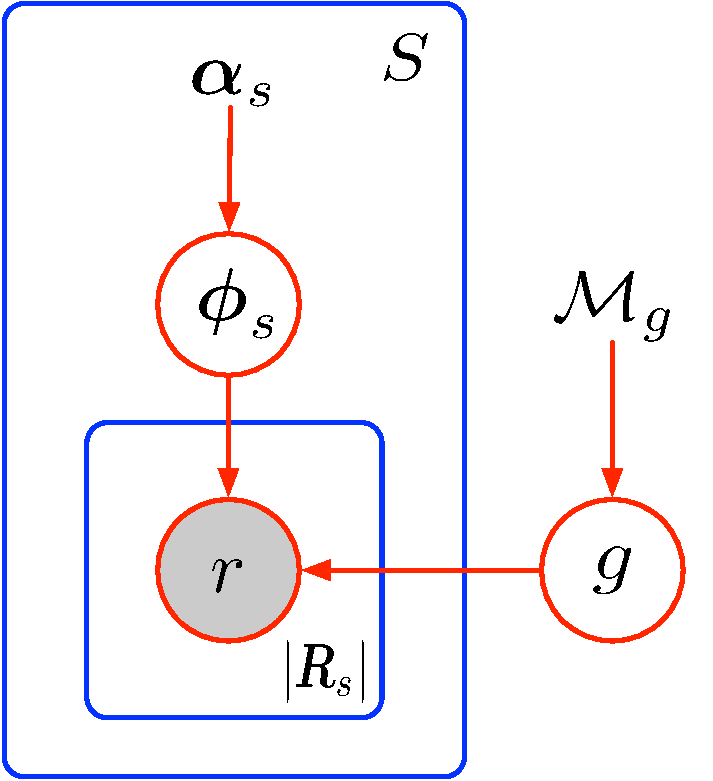
\includegraphics[width=0.3\textwidth]{figures/subclone_model}
\end{figure*}

\paragraph{Definitions}

\begin{center}
\begin{tabular}{ll}
Constants & Description \\
\hline
$P$ & The individuals genotype ploidy \\
$S$ & The number of samples for the individual \\
$G$ & The number of genotypes \\
$\boldsymbol{\phi}$ & Vector of $G$ probabilities \\
$g_{i}$ & The $j^{th}$ haplotype of the $i^{th}$ genotype \\
$\boldsymbol{\alpha_s}$ & A vector of $P$ Dirichlet counts \\
\hline
\end{tabular}
\end{center}

\begin{center}
\begin{tabular}{ll}
Observed latent variables & Description \\
\hline
$\mathcal{R}_s$ & The set of sequencing reads for sample $s$ of the individual \\
$N_s$ & $\mathcal{R}_s$ \\
\hline
\end{tabular}
\end{center}

\begin{center}
\begin{tabular}{ll}
Hidden latent variables & Description \\
\hline
$\boldsymbol{g}$ & Binary (1-of-$G$) \\
$\boldsymbol{\pi}_s$ & A vector of $P$ probabilities of sequencing each haplotype in the individuals genotype \\
$\boldsymbol{z}_{sn}$ & Binary (1-of-$P$), specifying which haplotype was sequenced in read $n$ of sample $s$ \\
\hline
\end{tabular}
\end{center}

\paragraph{Prior distributions}

There are two prior distributions in this model, the genotype prior $p(\boldsymbol{g} | \boldsymbol{\phi})$ and the haplotype mixture prior $p(\boldsymbol{\pi}_s | \boldsymbol{\alpha}_s)$ for $s = 1 \dots S$.

\paragraph{Marginal distributions}

The marginal distribution for $\boldsymbol{g}$ is categorical:

\begin{equation}
\label{eq:cnv_g_marginal}
    p(\boldsymbol{g} | \boldsymbol{\phi}) = \prod_{i = 1}^G \phi_i^{g_i}
\end{equation}

The marginal distribution of $\phi$ is assumed to be Dirichlet, this is mostly because it simplifies the mathematics.

\begin{equation}
\label{eq:cnv_pi_marginal}
    p(\boldsymbol{\pi} | \boldsymbol{\alpha}) = \text{Dir}(\boldsymbol{\pi} | \boldsymbol{\alpha}) = \frac{1}{\text{B}(\boldsymbol{\alpha})} \prod_{k = 1}^P \pi_k^{\alpha_k - 1}
\end{equation}

where $\text{B}(\boldsymbol{\alpha})$ is the multivariate Beta function:

\begin{equation}
\label{eq:beta_func}
    \text{B}(\boldsymbol{\alpha}) = \frac{\prod_{k = 1}^K \Gamma(\alpha_k)}{\Gamma(\sum_{k = 1}^K \alpha_k)}
\end{equation}

The marginal distribution for each $\boldsymbol{z}$ is categorical:

\begin{equation}
\label{eq:cnv_z_marginal}
    p(\boldsymbol{z} | \boldsymbol{\pi}) = \prod_{k = 1}^P \pi_k^{z_k}
\end{equation}

The marginal distribution for a single read $r$ is a mixture distribution:

\begin{align}
\label{eq:cnv_read_marginal}
 p(r | \boldsymbol{\pi}, g_i = 1) &= \sum_{\boldsymbol{z}} \sum^P_{k = 1} p(\boldsymbol{z} | \boldsymbol{\pi}) p(r | \boldsymbol{z}, h_{ik}) \\
 &= \sum^P_{k = 1} \pi_k p(r | h_{ik})
\end{align}

\paragraph{Joint distribution}

\begin{align}
\label{eq:cnv_jp}
 p(\mathcal{R}, \boldsymbol{g}, \boldsymbol{Z}, \boldsymbol{\pi} | \boldsymbol{\alpha}, \boldsymbol{\phi}) &= p(\boldsymbol{g} | \boldsymbol{\phi}) \prod_{s = 1}^S p(\boldsymbol{\pi}_s | \boldsymbol{\alpha}_s) p(\boldsymbol{Z}_s | \boldsymbol{\pi}_s) p(\mathcal{R}_s | \boldsymbol{Z}_s, \boldsymbol{g}) \\
 &= \prod^G_{i = 1} \phi_i^{g_i} \prod_{s = 1}^S \frac{1}{\text{B}(\boldsymbol{\alpha}_s)} \prod_{k = 1}^P \pi_{sk}^{\alpha_{sk} - 1} \prod_{n = 1}^{N_s} \prod_{k = 1}^P \pi_{sk}^{z_{snk}} \prod^G_{i = 1} \prod_{n = 1}^{N_s} \prod_{k = 1}^P p(r_{sn} | h_{ik})^{g_i z_{snk}}
\end{align}

\paragraph{Posterior distribution}

We are interested in the posterior distributions of $\boldsymbol{g}$ and $\boldsymbol{\pi}$, which due to the hidden latent variables $\boldsymbol{z}$ cannot be evaluated in closed form, we therefore resort to approximations. We choose a Variational Bayes approximation because it is deterministic and faster to compute than Monte Carlo based methods. A description of Variational Bayes is given in the appendix.

To evaluate approximate posterior distributions in the Variational Bayes framework we need to factorise (\ref{eq:cnv_jp}) into independent factors, there is only one possibility here:

\begin{equation}
\label{eq:cnv_vb_factors}
    q(\boldsymbol{g}, \boldsymbol{Z}, \boldsymbol{\pi}) = q(\boldsymbol{g}) \prod_{s = 1}^S q(\boldsymbol{Z}_s) q(\boldsymbol{\pi}_s)
\end{equation}

where non-latent variables have been omitted for brevity. We evaluate the optimal factors in tern.

\begin{align}
\label{eq:cnv_ln_q_z}
\ln q^*(\boldsymbol{Z}_s) &= \mathbb{E}_{\boldsymbol{g}, \boldsymbol{\pi}, \boldsymbol{Z}_{s' \ne s}} [\ln p(\mathcal{R}, \boldsymbol{g}, \boldsymbol{Z}, \boldsymbol{\pi} | \boldsymbol{\alpha}, \boldsymbol{\phi})] + \text{const} \\
&= \mathbb{E}[\ln p(\boldsymbol{Z}_s | \boldsymbol{\pi}_s)] + \mathbb{E}[\ln p(\mathcal{R}_s | \boldsymbol{Z}_s, \boldsymbol{g})] + \text{const} \\
&= \sum_{n = 1}^{N_s} \sum_{k = 1}^P z_{snk} \mathbb{E}[\ln \pi_{sk}] + \sum_{n = 1}^{N_s} \sum_{k = 1}^P \sum_{i = 1}^G z_{snk} \mathbb{E}[g_i] \ln p(r_{sn} | h_{ik}) + \text{const} \\
&= \sum_{n = 1}^{N_s} \sum_{k = 1}^P z_{snk} \ln \rho_{snk} + \text{const}
\end{align}

where we have defined

\begin{equation}
\label{eq:cnv_ln_rho}
\ln \rho_{snk} = \ln \tilde{\pi}_{sk} + \sum_{i = 1}^G \phi_i \ln p(r_{sn} | h_{ik})
\end{equation}

and

\begin{equation}
\label{eq:cnv_ex_ln_pi}
\ln \tilde{\pi}_{sk} = \psi(\alpha_{sk}) - \psi(\hat{\alpha}_s)
\end{equation}

where $\psi$ is the digamma function and $\hat{\alpha}_{s} = \sum_{k = 1}^P \alpha_{sk}$. Exponentiating both sides of (\ref{eq:cnv_ln_q_z}) and normalising we obtain:

\begin{equation}
\label{eq:cnv_q_z}
q^*(\boldsymbol{Z}_s) = \prod_{n = 1}^{N_s} \prod_{k = 1}^P \tau_{snk}^{z_{snk}}
\end{equation}

where

\begin{equation}
\label{eq:cnv_tau}
\tau_{snk} = \frac{\rho_{snk}}{\sum_{j = 1}^P \rho_{snj}}
\end{equation}

Next we look at each $q^*(\boldsymbol{\pi}_s)$:

\begin{align}
\label{eq:cnv_ln_q_pi}
\ln q^*(\boldsymbol{\pi}_s) &= \mathbb{E}_{\boldsymbol{g}, \boldsymbol{\pi}_s' \ne s}, \boldsymbol{Z} [\ln p(\mathcal{R}, \boldsymbol{g}, \boldsymbol{Z}, \boldsymbol{\pi} | \boldsymbol{\alpha}, \boldsymbol{\phi})] + \text{const} \\
&= \mathbb{E}[\ln p(\boldsymbol{\pi}_s | \boldsymbol{\alpha}_s)] + \mathbb{E}[\ln p(\boldsymbol{Z}_s | \boldsymbol{\pi}_s)] + \text{const} \\
&= \sum_{k = 1}^P (\alpha_k - 1) \ln \pi_{sk} + \sum_{k = 1}^P \sum_{n = 1}^{N_s} \tau_{snk} \ln \pi_{sk} + \text{const}
\end{align}

and therefore

\begin{align}
\label{eq:cnv_q_pi}
q^*(\boldsymbol{\pi}_s) &\propto \prod_{k = 1}^P \pi_{sk}^{\alpha_{sk} - 1} \prod_{k = 1}^P \pi_{sk}^{\sum_{n = 1}^{N_s} \tau_{snk}} \\
&=  \prod_{k = 1}^P \pi_{sk}^{\alpha_{sk} + \sum_{n = 1}^{N_s} \tau_{snk} - 1}
\end{align}

Which we can see from inspection is another Dirichlet distribution with pseudo-counts:

\begin{equation}
\label{eq:cnv_new_counts}
\alpha_{sk}^{post} = \alpha_{sk}^{prior} + \hat{N}_{sk}
\end{equation}

where $\hat{N}_{sk} = \sum_{n = 1}^{N_s} \tau_{snk}$. Finally we evaluate $q^*(\boldsymbol{g})$:

\begin{align}
\label{eq:cnv_ln_q_g}
\ln q^*(\boldsymbol{g}) &= \mathbb{E}_{\boldsymbol{\pi}, \boldsymbol{Z}} [\ln p(\mathcal{R}, \boldsymbol{g}, \boldsymbol{Z}, \boldsymbol{\pi} | \boldsymbol{\alpha}, \boldsymbol{\phi})] + \text{const} \\
&= \mathbb{E}[\ln p(\boldsymbol{g} | \boldsymbol{\phi})] + \mathbb{E}[\ln p(\mathcal{R}_s | \boldsymbol{Z}_s, \boldsymbol{g})] + \text{const} \\
&= \mathbb{E} \left [\sum_{i = 1}^G g_i \ln \phi_i \right] + \mathbb{E} \left[ \sum_{s = 1}^S \sum_{n = 1}^{N_s} \sum_{k = 1}^P \sum_{i = 1}^G g_i z_{snk} \ln p(r_{sn} | h_{ik}) \right] + \text{const} \\
&= \sum_{i = 1}^G \mathbb{E}[g_i] \ln \phi_i +  \sum_{i = 1}^G \mathbb{E}[g_i] \sum_{s = 1}^S \sum_{n = 1}^{N_s} \sum_{k = 1}^P \mathbb{E}[z_{snk}] \ln p(r_{sn} | h_{ik}) + \text{const} \\
&= \sum_{i = 1}^G \mathbb{E}[g_i] \left\{ \ln \phi_i + \sum_{s = 1}^S \sum_{n = 1}^{N_s} \sum_{k = 1}^P \tau_{snk} \ln p(r_{sn} | h_{ik}) \right\} + \text{const}
\end{align}

So we immediately see that

\begin{equation}
\label{eq:cnv_q_g}
q^*(\boldsymbol{g}) \propto \prod_{i = 1}^G \tilde{\phi}_i^{g_i}
\end{equation}

where

\begin{equation}
\label{eq:cnv_theta}
\ln \tilde{\phi}_i = \ln \phi_i + \sum_{n = 1}^{N_s} \sum_{k = 1}^P \tau_{snk} \ln p(r_{sn} | h_{ik})
\end{equation}

\paragraph{Evidence}

The Variational Bayes framework also gives a lower-bound on the evidence for the full posterior distribution. The lower bound is given by:

\begin{align}
\label{eq:cnv_evidence}
\begin{split}
\mathcal{L} &= \mathbb{E}[\ln p(\mathcal{R}, \boldsymbol{g}, \boldsymbol{Z}, \boldsymbol{\pi} | \boldsymbol{\alpha}, \boldsymbol{\phi})] - \mathbb{E} [\ln q^*(\boldsymbol{g}, \boldsymbol{Z}, \boldsymbol{\pi})] \\
&= \mathbb{E}[\ln p(\boldsymbol{g} | \boldsymbol{\phi})] + \sum_{s = 1}^S \left\{ \mathbb{E}[\ln p(\boldsymbol{\pi}_s | \boldsymbol{\alpha}_s)] + \mathbb{E}[\ln p(\boldsymbol{Z}_s | \boldsymbol{\pi}_s)] + \mathbb{E}[\ln p(\mathcal{R}_s | \boldsymbol{Z}_s, \boldsymbol{g})] \right\} \notag \\
     &\phantom{{}=\mathbb{E}[\ln p(\boldsymbol{g} | \boldsymbol{\phi})] } - \mathbb{E}[\ln q^*(\boldsymbol{g})] - \sum_{s = 1}^S \left\{ \mathbb{E}[\ln q^*(\boldsymbol{\pi}_s) + \mathbb{E}[\ln q^*(\boldsymbol{Z}_s)] \right\}
\end{split}
\end{align}

Where each expectation is taken with respect to $q^*$. Evaluating each term separately

\begin{equation}
\mathbb{E}[\ln p(\boldsymbol{g} | \boldsymbol{\phi})] = \mathbb{E}\left[\sum_{i = 1}^G g_i \ln \phi_i\right] = \sum_{i = 1}^G \mathbb{E}[g_i] \ln \phi_i = \sum_{i = 1}^G \phi_i^{post} \ln \phi_i^{prior}
\end{equation}

\begin{align}
\mathbb{E}[\ln p(\boldsymbol{\pi}_s | \boldsymbol{\alpha}_s)] &= \mathbb{E}\left[\sum_{k = 1}^P (\alpha_{sk}^{prior} - 1) \ln \pi_{sk} - \ln \text{B}(\boldsymbol{\alpha}_s^{prior})\right] \notag \\ 
&= \sum_{k = 1}^P (\alpha_{sk}^{prior} - 1) \mathbb{E} [\ln \pi_{sk}] - \ln \text{B}(\boldsymbol{\alpha}_s^{prior}) \notag \\
 &= \sum_{k = 1}^P (\alpha_{sk}^{prior} - 1) \ln \tilde{\pi}_{sk} - \ln \text{B}(\boldsymbol{\alpha}_s^{prior})
\end{align}

\begin{equation}
\mathbb{E}[\ln p(\boldsymbol{Z}_s | \boldsymbol{\pi}_s)] = \mathbb{E}\left[\sum_{n = 1}^{N_s} \sum_{k = 1}^P z_{snk} \ln \pi_{sk} \right] 
= \sum_{n = 1}^{N_s} \sum_{k = 1}^P \mathbb{E}[z_{snk} \ln \pi_{sk}]
= \sum_{n = 1}^{N_s} \sum_{k = 1}^P \tau_{snk} \ln \tilde{\pi}_{sk}
\end{equation}

as $\tau$ and $z$ are independent under $q$.

\begin{equation}
\mathbb{E}[\ln p(\mathcal{R}_s | \boldsymbol{Z}_s, \boldsymbol{g})] = \mathbb{E}\left[ \sum_{i = 1}^G \sum_{n = 1}^{N_s} \sum_{k = 1}^P g_i z_{snk} \ln p(r_{sn} | h_{ik}) \right] = \sum_{i = 1}^G \phi_i^{post} \sum_{n = 1}^{N_s} \sum_{k = 1}^P \tau_{snk} \ln p(r_{sn} | h_{ik})
\end{equation}

\begin{equation}
\mathbb{E}[\ln q^*(\boldsymbol{g})] = \mathbb{E}\left[\sum_{i = 1}^G g_i \ln \tilde{\phi}_i\right] = \sum_{i = 1}^G \mathbb{E}[g_i] \ln \tilde{\phi}_i = \sum_{i = 1}^G \phi_i^{post} \ln \phi_i^{post}
\end{equation}

\begin{align}
\mathbb{E}[\ln q^*(\boldsymbol{\pi}_s)] =& \mathbb{E}\left[\sum_{k = 1}^P (\alpha_{sk}^{post} - 1) \ln \pi_{sk} - \ln \text{B}(\boldsymbol{\alpha}_s^{post})\right] \notag \\ 
&= \sum_{k = 1}^P (\alpha_{sk}^{post} - 1) \mathbb{E} [\ln \pi_{sk}] - \ln \text{B}(\boldsymbol{\alpha}_s^{post}) \notag \\
 &= \sum_{k = 1}^P (\alpha_{sk}^{post} - 1) \ln \tilde{\pi}_{sk} - \ln \text{B}(\boldsymbol{\alpha}_s^{post})
\end{align}

\begin{equation}
\mathbb{E}[\ln q^*(\boldsymbol{Z}_s)] = \mathbb{E}\left[\sum_{n = 1}^{N_s} \sum_{k = 1}^P z_{snk} \ln \tau_{snk} \right] = \sum_{n = 1}^{N_s} \sum_{k = 1}^P \tau_{snk} \ln \tau_{snk}
\end{equation}

After a little algebra we get:

\begin{equation}
\mathcal{L} = \sum_{i = 1}^G \phi_i^{post}\left\{ \ln \frac{\phi_i^{prior}}{\phi_i^{post}} + \sum_{s = 1}^S \sum_{n = 1}^{N_s} \sum_{k = 1}^P \tau_{snk} \ln p(r_{sn} | h_{ik}) \right\} + \sum_{s = 1}^S \left\{ \ln \frac{\text{B}(\boldsymbol{\alpha}_s^{post})}{\text{B}(\boldsymbol{\alpha}_s^{prior})} + \text{H}[\boldsymbol{Z}_s] \right\}
\end{equation}

where $\text{H}$ is entropy in nats.

\subsection{Calling models}\label{calling-models}

Calling models are the heart of Octopus. The are ultimately responsable for all variant and genotype calls made, phasing (as they infer the genotype posterior distribution used for phasing), and any other inferences that may be reported with variant calls. In addition to variant calls, calling models must be able to report a posterior probability distribution over genotypes (for each sample) and haplotypes (over all samples). The former is used for phasing, the latter for haplotype filtering. All calling models make use of one or more genotype models (\ref{model:genotype-posterior}).

\subsubsection{Individual}\label{caller:individual}

\paragraph{Overview}

The individual calling model is the simplest calling model. It considers a single individual with known ploidy and copy number.

\paragraph{Genotype generation}

All possible genotypes are considered given the set of haplotypes, $\boldsymbol{h}$, and sample ploidy, $P$. There are

\begin{equation}
\binom{|\boldsymbol{h}| + P - 1}{|\boldsymbol{h}| - 1}
\end{equation}

possible genotypes.

\paragraph{Inference: genotype posteriors}

Unsurprisingly, the individual calling model uses the individual genotype model (\ref{genotype-model:individual}) for inference. Fitting the individual genotype model is cheap and can be done exactly.

\paragraph{Inference: haplotype posteriors}

The haplotype posterior distribution is computed by marginalising over the genotype posterior distribution:

\begin{equation}
p(h | \mathcal{R}) = \sum_{g : \boldsymbol{g}} [h \in g]p(g | \mathcal{R})
\end{equation}

where $h \in g$ is true if $h$ occurs in $g$ at least once.

\paragraph{Inference: variant and genotype calls}\label{calling:individual-variants}

First we calculate the posterior probability of all candidate non-reference alleles by marginalising over the genotype posterior distribution:

\begin{equation}
p(a | \mathcal{R}) = \sum_{g : \boldsymbol{g}} [a \in g]p(g | \mathcal{R})
\end{equation}

where $a \in g$ is true if the $\text{any}(a \in h) \text{for} h : g$ (i.e. if $a$ occurs in any of the haplotypes in $g$). We then select alleles with posterior probability above some user-specified threshold.

Next, we identify the genotype with the greatest posterior probability (i.e. the MAP genotype). All selected alleles that appear on the MAP genotype are called variants, where the variant quality is determined by the marginalised allele posterior computed previously.

For each called allele, we then call genotypes at the loci of those alleles. In particular, for an allele $a$ we identify the alleles present in the called genotype at that loci, and once again marginalise over the genotype posterior distribution to compute the posterior probability for that local genotype. This is used for the genotype quality score.

\subsubsection{Population}

\paragraph{Overview}
\paragraph{Genotype generation}
\paragraph{Inference: genotype posteriors}
\paragraph{Inference: haplotype posteriors}
\paragraph{Inference: variant and genotype calls}

\subsubsection{Trio}

\paragraph{Overview}

The trio genotype model is intended for calling germline and \textit{de novo} variants in parent-offspring trios. Since we know the relationship between the parental samples and the child, we include this knowledge directly in the genotype prior model (\ref{model:trio-prior}).

\paragraph{Genotype generation}

We generate all possible genotypes for the mother, father, and child, given the candidate haplotypes, $\boldsymbol{h}$, and sample ploidies, $P_m, P_p, P_o$ for the mother, father, and child respectively. Then there are:

\begin{equation}
G_m = \binom{|\boldsymbol{h}| + P_m - 1}{|\boldsymbol{h}| - 1} \quad G_p = \binom{|\boldsymbol{h}| + P_p - 1}{|\boldsymbol{h}| - 1} \quad G_o = \binom{|\boldsymbol{h}| + P_o - 1}{|\boldsymbol{h}| - 1}
\end{equation}

genotypes, where $G_m, G_p, G_o$ is for the mother, father, and child respectively. If samples have the same ploidy then they share genotypes.

\paragraph{Inference: genotype posteriors}

We evaluate the trio genotype posterior model (\ref{model:trio}). The total number of possible joint genotypes we consider is $G = G_m \times G_p \times G_o$. If the number of candidate haplotypes is large, then $G$ could be very large. For example, if $|\boldsymbol{h}| = 200$ (the default maximum) and all samples are diploid then $G = 8,120,601,000,000$. Even if we could evaluate one combination per microsecond, it would take around $90$ days to evaluate the full genotype prior. Clearly this is not pratical; we must only consider a small subset of the possible combinations. We adopt the following strategy:

\begin{enumerate}
	\item Set the maximum number of joint genotype evaluations to $\tau_G$, and $\tau' = \sqrt{\tau_G}$.
	\item Set the target 'loss' in probability mass to $\epsilon$.
	\item Calculate genotype likelihoods for each sample.
	\item For each sample $s$, find a subset of genotypes $\boldsymbol{g}'_s$: 
	\begin{enumerate}
		\item Evaluate a posterior distribution for the samples genotypes under a uniform prior genotype model (\ref{model:uniform}).
		\item Sort the samples genotypes under the uniform genotype posterior.
		\item If the sum of the $\tau'$ highest posterior genotypes is greater than $\epsilon$ then use these genotypes.
		\item Evaluate the genotype posterior distribution with the provided germline genotype prior model and use the top $\tau'$ genotypes.
	\end{enumerate}
	\item Find a subset of parental genotype combinations, $\boldsymbol{g'_{mp}}$, using $\boldsymbol{g'_{m}}$ and $\boldsymbol{g'_{p}}$:
	\begin{enumerate}
		\item 
	\end{enumerate}
	\item Evaluate posteriors using the trio prior model for $\boldsymbol{g'_{mp}}$ and $\boldsymbol{g'_o}$
\end{enumerate}

The trio genotype posterior model inferes a posterior distribution over genotype combinations, but it is simple to compute marginal sample genotype posteriors by integrating over the genotypes of the other two samples, for example, the offspring marginal posterior is:

\begin{equation}
p(g_o | \mathcal{R}) = \sum_{(g_m, g_p, g'_o) \in \boldsymbol{g}} [g'_o = g_o] p(g_m, g_p, g'_o | \mathcal{R})
\end{equation}

\paragraph{Inference: haplotype posteriors}

We calculate posterior probability a haplotype, $h$, is segregating in the trio by integrating over the posterior marginal distribution:

\begin{equation}
p(h | \mathcal{R}) = 1 - \prod_{s \in \{m, p, o\}}\sum_{g_s : \boldsymbol{g}_s} [h \notin g]p(g_s | \mathcal{R})
\end{equation}

\paragraph{Inference: variant and genotype calls}

To calculate the probability an allele segregates in the trio, we integrate over the joint genotype posterior distribution:

\begin{equation}
p(a | \mathcal{R}) = 1 - \prod_{s \in \{m, p, o\}}\sum_{g_s : \boldsymbol{g}_s} [a \notin g]p(g_s | \mathcal{R})
\end{equation}

Similarly, we calculate the posterior probability an allele is \textit{de novo} in the child:

\begin{equation}
p_{denovo}(a | \mathcal{R}) = \sum_{(g_m, g_p, g_o) \in \boldsymbol{g}} [a \notin g_m \land a \notin g_p \land a \in g_o] p(g_m, g_p, g_o | \mathcal{R})
\end{equation}

Next, we find the MAP genotype combination. 

\subsubsection{Cancer}

\paragraph{Overview}

The cancer caller is intended to detect somatic mutations in a set of tumour samples from a single individual. The set of samples may also include samples that are not expected to contain somatic mutations (i.e. normal samples). It should always be possible to combine normal samples, so we just assume one normal sample may be present. We must be aware of resulting from cancer biology and experiemntal design we expect to observe:

\begin{itemize}
	\item There are no somatic mutational events; reads are generated from a clean germline.
	\item Somatic copy number changes have occurred.
	\item Somatic mutations have occurred.
\end{itemize}

We must also consider that if somatic events have occurred, there may still be reads generated from healthy cells.

The cancer calling model makes use of two genotype posterior models: the individual model (\ref{genotype-model:individual}) and the subclone model (\ref{model:subclone}). Two instances of the subclone model are used, one with a \emph{germline} genotype prior model (e.g. the coalescent-HWE model (\ref{model:coalescent-hwe})), and another with a \emph{cancer} genotype prior model (\ref{model:cancer-prior}).

\paragraph{Genotype generation}

We generate all possible germline genotypes given the sample ploidy, $P$, and set of candidate haplotypes, $\boldsymbol{h}$ and apply the individual calling model. We also generate \emph{cancer} genotypes which were discussed in the cancer genotype prior model section (\ref{model:cancer-prior}). Initially we generate all possible cancer genotypes with somatic ploidy 1.

\paragraph{Model fitting}



\paragraph{Model comparison}

We then fit the individual $\mathcal{M}_g$, CNV $\mathcal{M}_c$, and somatic $\mathcal{M}_s$ models to the data. For the individual case all reads are pooled together, which as can be seen from \ref{eq:ind_jp} results in the same likelihood function as treating each sample separately. We then calculate the posterior probability of each model by evaluating Bayes theorem:

\begin{equation}
\label{eq:bayes_model}
p(\mathcal{M} | \mathcal{D}) = \frac{p(\mathcal{M})p(\mathcal{D} | \mathcal{M})}{p(\mathcal{D})}
\end{equation}

In particular the term $p(\mathcal{D} | \mathcal{M})$  is the evidence the model $\mathcal{M}$, and $p(\mathcal{M})$ is the prior probability.

\paragraph{Germline genotype calling}

The probability of each germline genotype is then:

\begin{equation}
\label{eq:som_germline_genotype}
p(\boldsymbol{g} | \mathcal{R}) = p(\mathcal{M}_g | \mathcal{R}) p(\boldsymbol{g} | \mathcal{M}_g) + p(\mathcal{M}_c | \mathcal{R}) p(\boldsymbol{g} | \mathcal{M}_c) + p(\mathcal{M}_s | \mathcal{R}) p(\boldsymbol{g} | \mathcal{M}_s)
\end{equation}

\noindent where $p(\boldsymbol{g} | \mathcal{M}_s) = \sum_{\tilde{\boldsymbol{g}} s.t. \boldsymbol{g} \in \tilde{\boldsymbol{g}}} p(\tilde{\boldsymbol{g}} | \mathcal{M}_s)$.

The called genotype is then the MAP genotype according to this posterior distribution.

\paragraph{Germline variant calling}

The posterior probability of each candidate variant allele $a$ is then:

\begin{equation}
\label{eq:som_germline_candidate}
p(a | \mathcal{R}) = \sum_{\boldsymbol{g} s.t. a \in \boldsymbol{g}} p(\boldsymbol{g} | \mathcal{R})
\end{equation}

Germline candidates are called if the posterior is above a user defined threshold, and if the candidate is present in the called germline genotype. If the candidate is not above the user-defined threshold, it is added to a list of candidate somatic candidates.

\paragraph{Somatic allele calling}

Noting that $\mathcal{M}_s$ defines a probability distribution of probabilities over each component of each samples 'cancer genotype', we define the probability that a particular sample contains a somatic haplotype, $\tilde{h}$, as:

\begin{equation}
\label{eq:somatic_probability_sample}
p(\tilde{h}_s | \mathcal{M}_s) = p(\tilde{h}_s > c_s | \mathcal{M}_s) = \int_c^1 \text{Beta}(\alpha_{P + 1}, \sum_{i = 0}^{P} \alpha_i)
\end{equation}

\noindent where $c_s$ is some user-defined threshold. The idea being somatic haplotypes with most probability mass less than $c_s$ are considered noise.

We can then calculate the probability that a somatic haplotype is present in any of the samples as:

\begin{equation}
\label{eq:somatic_probability}
p(\tilde{h} | \mathcal{M}_s) = 1 - \prod_s 1 - p(\tilde{h}_s | \mathcal{M}_s)
\end{equation}

\noindent If this probability is greater than some user-defined threshold, we proceed to call somatic mutations.

\subsubsection{Polyclone}

\paragraph{Overview}

The polyclone calling model is intended to identify variants in a single sample of mixed haploid clones. Such samples commonly arise in bacterial or viral sequencing due to mixed infection. in-host evolution, or sample contamination. In addition to the number of clones in the sample being unknown \textit{a priori}, the frequency of clones as a function of the number is also unknown. The problem is very similar to calling a single tumour sample, but in the polyclone model, all variants are considered germline, so there is no attempt to classify calls as somatic.

\paragraph{Genotype generation}

We start by generating all possible haploid and diploid genotypes given the candidates haplotypes, $\boldsymbol{h}$. There are $|\boldsymbol{h}|$ haploid genotypes and $\binom{|\boldsymbol{h}| + P1}{|\boldsymbol{h}| - 1}$ diploid genotypes.

\paragraph{Model fitting}

First, We evaluate the individual genotype posterior model (\ref{genotype-model:individual}) for the haploid genotypes, and the subclone  genotype posterior model (\ref{model:subclone}) for the diploid genotypes. If the diploid model evidence is greater than the haploid model evidence, then we generate all triploid genotypes and evaluate the subclone model with these genotypes. We continue in this fashion until the model evidence decreases, or a user-specified ploidy limit is reached. We can also include a model prior that is a function of the ploidy. The ploidy with the greatest model posterior is used for inference.

\paragraph{Inference: genotype posteriors}

We use the genotype posterior distribution of the model with the highest evidence $\mathcal{M}^*$, the associated candidate genotypes are $\boldsymbol{g}^*$.

\paragraph{Inference: haplotype posteriors}

The haplotype posterior distribution is computed by marginalising over the genotype posterior distribution:

\begin{equation}
p(h | \mathcal{R}, \mathcal{M}^*) = \sum_{g : \boldsymbol{g}^*} [h \in g]p(g | \mathcal{R}, \mathcal{M}^*)
\end{equation}

where $h \in g$ is true if $h$ occurs in $g$ at least once.

\paragraph{Inference: variant and genotype calls}

Variant and genotype calls are made in the same way as for the individual calling model (\ref{calling:individual-variants}).

\subsection{Variant phasing}\label{phasing}

Although each caller implements different genotype models, each is required to infer the marginal posterior probability of genotypes for each sample (\ref{calling-models}). This posterior distribution is used to infer physical phasing of called variant sites. Direct read data is not required as all information available from the reads, in addition to any prior information, is already contained in the posterior distribution. The advantage of this approach is exemplified when calling trios as the genotype prior can be strongly informative about phase due to identity by decent. The method applies to genotypes of arbitrary zygosity and is therefore applicable to non-diploid samples.

Samples are phased independently; the marginal genotype posterior distribution for each sample is used for phasing. First, all genotypes in the domain of the posterior distribution are partitioned into phase complement sets. All genotypes in a phase complement set share exactly the same alleles, but may appear on different haplotypes. There is only one such partitioning possible for any set of genotypes. An example of a phase set partition is shown in Figure \ref{fig:phase-sets}.

\begin{figure}[ht]
    \centering
	\label{fig:phase-sets}
    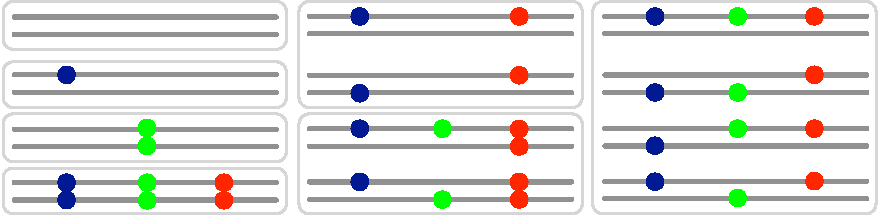
\includegraphics[width=0.8\textwidth]{figures/phase-sets}
	\caption{The phase complement sets for 12 diploid genotypes comprised of 9 unique haplotypes and 6 alleles. Non-reference alleles are coloured dots and grey bars are haplotypes. The first column shows four distinct phase complement sets with a single genotype in each. The second column shows two phase complement sets with two genotypes in each. The last column has a single phase complement set with four genotypes. Note that the key property that defines the phase complement sets is that the genotypes at each allele loci are all the same for each genotype within the set.}
\end{figure}

We calculate the entropy of each set with respect to the normalised posterior probabilities of the genotypes contained in the set. A low entropy implies little uncertainty in the phase of the alleles present in the set. To account for uncertainty in the samples genotype, we marginalise over all phase complement sets by taking the weighted sum of each sets entropy, where the weight for each set is the sum of the unnormalised posterior probabilities. We termed this weighted average a phase score.

\begin{equation}
    \text{PS}(\boldsymbol{g} | \mathcal{R}_s) = \sum_j \tau_j H\left(\left[\frac{p(g_{j0} | \mathcal{R}_s)}{\tau_j}, ..., \frac{p(g_{jm}| \mathcal{R}_s)}{\tau_j}\right]\right)
\end{equation}

Lower phase scores indicate less ambiguous phasing, even if there is high uncertainty in the samples genotype. If the phase score for a set of genotypes is lower than a given threshold the region is considered phased, otherwise, each genotype in the set can be broken into two parts which results in two unphased sets of partial genotypes. The phase scores of these two partial sets is never greater than the phase score of the original genotype set. The phasing algorithm therefore iteratively finds the smallest set of breakpoints such that the partial genotype sets defined by those breakpoints are all phased.


\subsection{Variant filtering}

As with any model, there are some error modes that are not well captured by Octopus’ calling models which can lead to false inferences. For example, Octopus assumes read sequencing and mapping errors are independent which is not true in general. To identify false calls due to model error, we developed classifiers to filter Octopus’s raw calls using statistics (called measures in Octopus) that may be derived directly from the input read data.

\subsubsection{Measures}

The current available measures are:

\begin{center}
\begin{tabular}{lll}
Label & Description & Sample specific? \\
\hline
AC & Number of called non-reference alleles & Yes \\
AD & Minor empirical non-reference allele depth & Yes \\
AF & Minor empirical non-reference allele frequency & Yes \\
ARF & Fraction of reads that cannot be assigned to a unique called haplotype & Yes \\
BQ & Minimum median base quality of reads supporting each allele & Yes \\
CRF & Fraction of soft clipped reads covering the site & No \\
DC & Number of reads supporting a called \textit{de novo} haplotype in the offsprings parents & Yes \\
DENOVO & Is the call a \textit{de novo} mutation? & No \\
DP & Read depth at the site & Yes \\
FRF & Fraction of reads filtered for calling at the site & Yes \\
GC & G + C fraction of reference around the site & No \\
GQ & Called genotype quality GQ & Yes \\
GQD & GQ divided by DP & Yes \\
MC & Number of reads with mismatch at site in reads supporting variant haplotype  & Yes \\
MF & Fraction of reads with mismatch at site in reads supporting variant haplotype  & Yes \\
MP & Model Posterior calculated by octopus's calling model & No \\
MQ & Median mapping quality of reads overlapping the site & No \\
MQ0 & Number of reads with mapping quality zero overlapping the site & No \\
QUAL & Quality of the call & No \\
QD & QUAL / sum(DP for each sample) & No \\
REFCALL & Is the call homozygous reference? & Yes \\
RPB & Bias of variant w.r.t read position (head or tail) & Yes \\
SB & Strand bias of non-reference alleles & Yes \\
SD & Strand bias of reads overlapping the site; probability mass in tails of Beta distribution & Yes \\
SC & Number of reads supporting a called somatic haplotype in somatic samples & Yes \\
SHC & Number of called somatic haplotypes & Yes \\
SMQ & Median mapping quality of reads assigned to called somatic haplotypes & Yes \\
SOMATIC & Is the call a somatic mutation? & Yes \\
STR\_LENGTH & Length of STR overlapping the site & No \\
STR\_PERIOD & Period of STR overlapping the site & No \\
\hline
\end{tabular}
\end{center}

\subsubsection{Threshold filters}

Threshold filters are Boolean expressions where the terms of the expression are comparison operations. Currently, only \emph{or} binary operations are permitted; if any of the individual operations is true then the call is filtered. However, it would not be difficult to extend this to more general Boolean expressions.

\subsubsection{Random forest filters}

Random forests are a powerful machine learning method that can be used for both regression and classification. They are well suited to variant calling as most false positive calls will likely originate from a low-dimensional subspace of error modes. A nice feature of classification random forests is that they are able to report a measure of confidence in each class for a given input, which may be interpreted as a probability. This score is a useful single value for the quality of a call given the classification criteria.

\subsection{Realigned evidence BAMs}\label{bam-realignments}

Octopus is capable of producing realigned BAM files that provide further evidence of a calls reliability. These BAM files are especially helpful in cases where there are complex indel variants and the input alignments are significantly different from the alignments supported by the called haplotypes. For each read, there are four steps:

\begin{enumerate}
	\item Identify the called haplotype where the read originated from.
	\item Align the haplotype to the reference sequence.
	\item Align the read to the haplotype (mismatches due to sequencing or calling errors).
	\item Merge the two alignments to obtain a single alignment to the reference.
\end{enumerate}

For the first step, we use the called haplotype that has the maximum likelihood of generating the read. If there are more than one haplotype that have equal likelihood, then we call the read \emph{ambiguous}. For the purpose of BAM realignment, ambiguous are assigned randomly to one of the equally well supported haplotypes. The second step is trivial in Octopus since haplotypes are defined explicitly by alleles that are reported in the VCF output. The third step is also trivial; we just use the Viterbi alignment found from calculating the maximum likelihood in the first step. The final step is tricky if the alignment found in the third step has indel mismatches. We always try to report an alignment that has the fewest number of CIGAR operations.

Since Octopus makes a hard choice of called haplotype in the first step, it is also possible to report this information in the BAM output. One way to do this would be to tag the read with this information. While we will look to implement this in the future, another simple way is to produce separate BAM files for each of the called haplotypes in the sample. Octopus is also capable of producing these 'split' realigned BAMs.

\section{Results}

\subsection{Germline calling}

\subsubsection{Data}

Whole genome germline calls were made using sequencing data derived from the well studied individual NA12878. We found four sequencing libraries for NA12878, three high coverage and one low coverage, for evaluation:

\begin{enumerate}
    \item High coverage Illumina reads from the 1000G phase 3 project, Aligned reads were downloaded from \url{ftp.1000genomes.ebi.ac.uk:/vol1/ftp/phase3/data/NA12878/high_coverage_alignment/NA12878.mapped.ILLUMINA.bwa.CEU.high_coverage_pcr_free.20130906.bam}.
    \item Low coverage Illumina reads from the 1000G phase 3 project. Aligned reads were downloaded from \url{ftp.1000genomes.ebi.ac.uk:/vol1/ftp/phase3/data/NA12878/alignment/NA12878.mapped.ILLUMINA.bwa.CEU.low_coverage.20121211.bam}.
    \item High coverage Illumina reads from the Illumina Platinum Genomes project. Raw FASTQ files were downloaded from \url{https://storage.cloud.google.com/genomics-public-data/platinum-genomes/fastq/ERR194147_1.fastq.gz?_ga=2.121231755.-2019438195.1508521573} and \url{https://storage.cloud.google.com/genomics-public-data/platinum-genomes/fastq/ERR194147_2.fastq.gz?_ga=2.134461938.-2019438195.1508521573}.
    \item High coverage Illumina X Ten reads. Raw FASTQ files were downloaded from \url{https://s3-ap-southeast-2.amazonaws.com/kccg-x10-truseq-nano-v2.5-na12878/NA12878_V2.5_Robot_2_R1.fastq.gz} and \url{https://s3-ap-southeast-2.amazonaws.com/kccg-x10-truseq-nano-v2.5-na12878/NA12878_V2.5_Robot_2_R2.fastq.gz}.
\end{enumerate}

\subsubsection{Commands}

\subsubsection{Evaluation}

\subsection{\textit{De novo} calling}

\subsection{Synthetic tumour generation}

\subsection{Paired somatic calling}

\subsection{Unpaired somatic calling}

\section{Appendix}

\subsection{Variational Bayes}

Given a probability model $p(\boldsymbol{X}, \boldsymbol{Z})$ where $\boldsymbol{X}$ is observed and $\boldsymbol{Z}$ are latent, the true posterior density $p(\boldsymbol{Z} | \boldsymbol{X})$ can be approximated with another distribution $q(\boldsymbol{Z})$ subject to some measure of similarity. A natural choice of similarity is the Kullback–Leibler divergence

\begin{equation}
\label{eq:kl}
   \text{KL} (q\; ||\; p) = -\int q(\boldsymbol{Z}) \ln \frac{p(\boldsymbol{Z} | \boldsymbol{X})}{q(\boldsymbol{Z})} d\boldsymbol{Z}
\end{equation}

This measures the additional amount of information (in nats) required to generate codes from $q$ rather than $p$, it satisfies $\text{KL}(q\; ||\; p) \ge 0$, with equality when $p = q$. So we actually try to minimise this quantity.

We now partition the latent variables $\boldsymbol{Z}$ into a set of disjoint groups denoted by $\boldsymbol{Z_i}$ where $i = 1, \dots, M$ and assume that the $q$ distribution factorises into a product of these groups, i.e.

\begin{equation}
\label{eq:q}
  q(\boldsymbol{Z}) = \prod_{i = 1}^M q_i(\boldsymbol{Z_i})
\end{equation}

This is the only assumption made, in particular the functional form of each $q_i$ is not constrained. The idea is then to optimise each group in tern, which can formally be solved using calculus of variations, but we can to see that by substituting (\ref{eq:q}) into (\ref{eq:kl}) and separating one group $\boldsymbol{Z_j}$ that

\begin{align}
    \text{KL}(q\; ||\; p) &= -\int \prod_{i = 1}^M q_i \left\{ \ln p(\boldsymbol{Z} | \boldsymbol{X}) - \sum_i \ln q_i) \right\} d \boldsymbol{Z}\notag \\
    &= -\int q_j \left\{ \int \ln p(\boldsymbol{Z} | \boldsymbol{X}) \prod_{i \ne j} d \boldsymbol{Z_i} \right\} d \boldsymbol{Z_j} + \int q_j \ln q_j d \boldsymbol{Z_j} + \text{const}\notag\\
    &= -\int q_j \mathbb{E}_{i \ne j}[\ln p(\boldsymbol{Z} | \boldsymbol{X})] d \boldsymbol{Z_j} + \int q_j \ln q_j d \boldsymbol{Z_j} + \text{const}\notag\\
    &= \text{KL}(q_j\; ||\; \exp (\mathbb{E}_{i \ne j}[\ln p(\boldsymbol{Z} | \boldsymbol{X})])) + \text{const}
\end{align}

Clearly the $q_j$ which minimises this quantity is when $q_j = \exp(\mathbb{E}_{i \ne j}[\ln p(\boldsymbol{Z} | \boldsymbol{X})])$ and therefore we find the optimal $q_j$

\begin{equation}
q^*_j(\boldsymbol{Z_j}) = \mathbb{E}_{i \ne j}[\ln p(\boldsymbol{Z} | \boldsymbol{X})] + \text{const}
\end{equation}

or equivalently if $p(\boldsymbol{X})$ is absorbed into the constant then

\begin{equation}
\label{eq:q_opt}
q^*_j(\boldsymbol{Z_j}) = \mathbb{E}_{i \ne j}[\ln p(\boldsymbol{X}, \boldsymbol{Z})] + \text{const}
\end{equation}

Note these equations do not represent an explicit solution because they are interdependent. The variational Bayes algorithm therefore proceeds similar to EM by cycling through each group, updating $q^*$, and repeating until convergence. It can be shown that $\text{KL}(q\; ||\; p)$ decreases at each step.

\end{document}
